\begin{figure}[p]
\centering
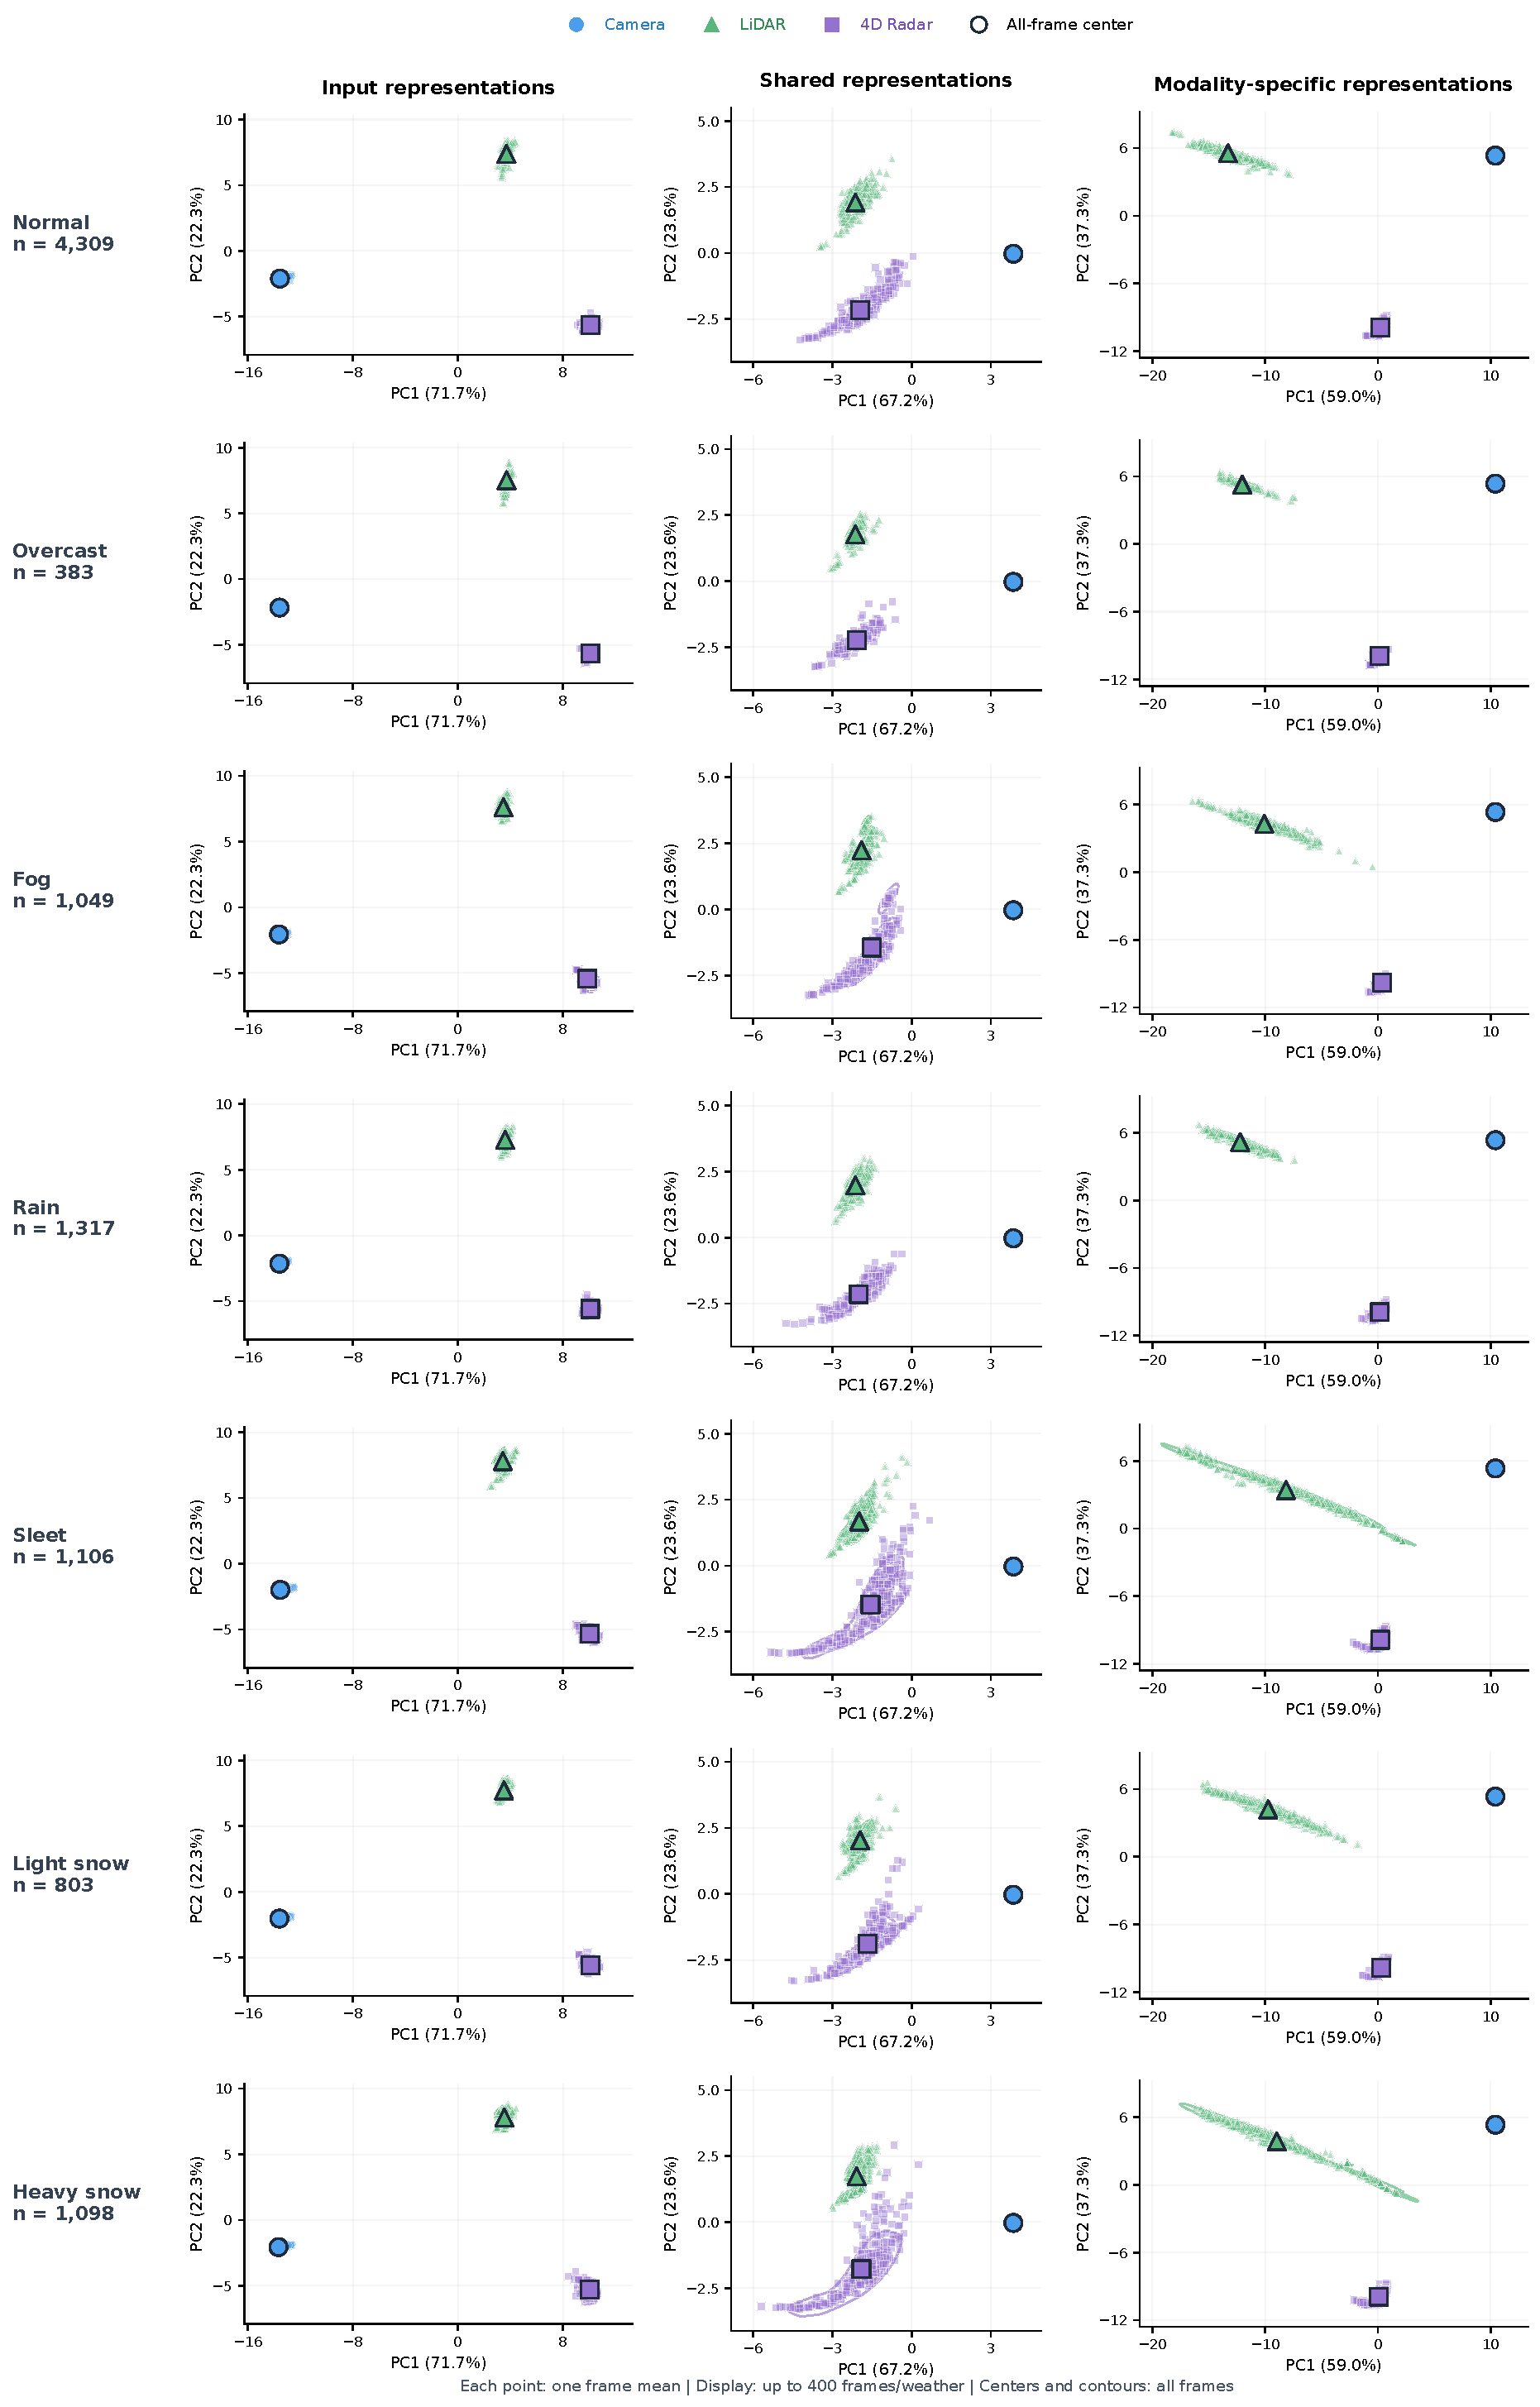
\includegraphics[width=\linewidth,height=.69\textheight,keepaspectratio]{assets/pca_all_weather.pdf}
\caption{Frame-level representation distributions over the complete K-Radar v1 test set. Rows indicate weather groups; columns show input, shared, and modality-specific representations. Each point is a frame's mean vector over GT foreground locations, projected using the fixed weighted PCA basis for its column. Blue circles, green triangles, and purple squares denote camera, LiDAR, and 4D radar. Up to 400 frames are displayed per group, including all 383 overcast frames. Large outlined markers and density contours use all frames, and n denotes the full group size. Each column shares its basis and axis ranges across weather; columns are fitted independently. Residual modality structure in these projections and high-dimensional cosine consistency in Table~\ref{tab:e1} characterize different properties.}
\label{fig:e1}
\end{figure}
